\documentclass[brazil]{beamer}
\usepackage[brazilian]{babel}
\usepackage[utf8]{inputenc}
\usepackage{graphics}
\usepackage{listings}
\usetheme{Szeged}
\usecolortheme{whale}

\title{Comparação de eficiência entre OpenCL e CUDA}
\author{Thiago de Gouveia Nunes}

\begin{document}

\lstset{
basicstyle=\small,
identifierstyle=, 
stringstyle=\ttfamily,
showstringspaces=false,
language=c,
keywordstyle=\color{blue}}

\frame{\titlepage}

%-------------------------------------
\section{Tecnologias}
%-------------------------------------

\frame{
  \frametitle{GPGPU}
  É usar uma GPU (Graphics Processing Unit), uma placa criada com foco em Computação Gráfica, 
  para processamento de propósito geral.
}

\frame{
  \frametitle{GPGPU}
  Existem 2 linguagens fortes no mercado para GPGPU, o \textbf{CUDA} (Compute Unified Device Architecture) feita pela
  \textit{NVIDIA}, e o \textbf{OpenCL} (Open Computing Language) feito pelo Khronos Group, o mesmo grupo responsável pelo
  OpenGL. O objetivo do trabalho é comparar esses dois frameworks através de testes de desempenho e comparação nas abstrações
  feitas para utilizar a GPU.
}

\frame{
  \frametitle{OpenCL}
    \begin{columns}
      \begin{column}{.5\textwidth}
        
\includegraphics[scale=0.7]{OpenCL_Logo.png}
      \end{column}
      \begin{column}{.5\textwidth}
         O OpenCL é uma linguagem de programação paralela para sistemas híbridos. O OpenCL iniciativa open source da Apple.
          Hoje ela é mantida pelo grupo Khronos.
      \end{column}
    \end{columns}
}

\frame{
  \frametitle{CUDA}
  \begin{columns}
    \begin{column}{.5\textwidth}
      
\includegraphics[scale=0.3]{CUDAlogo.jpg}
    \end{column}
    \begin{column}{.5\textwidth}
      CUDA é uma linguagem proprietária para programação paralela em GPUs desenvolvida pela NVIDIA. 
      Atualmente só existe 1 compilador de CUDA para placas NVIDIA, o \textit{nvcc}.
    \end{column}
  \end{columns}
  
}

\frame{
  \frametitle{GPU}
  \begin{columns}
    \begin{column}{.6\textwidth}
  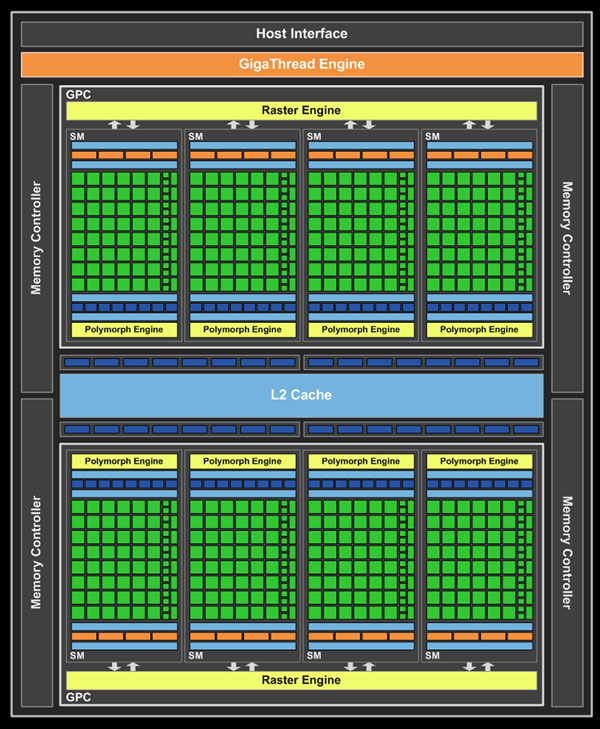
\includegraphics[scale=0.28]{15596_large_GTX460_Architecture.jpg}  
    \end{column}
    \begin{column}{.4\textwidth}
  Antes de entrar na comparação entre as linguagens, vamos discutir sobre a arquitetura da GPU usada para os testes, 
  uma GeForce GTX 460 SE.
    \end{column}
  \end{columns}
}

\begin{frame}[fragile]
  \frametitle{Arquitetura GeForce GTX 460 SE}
  \begin{columns}
    \begin{column}{.5\textwidth}
      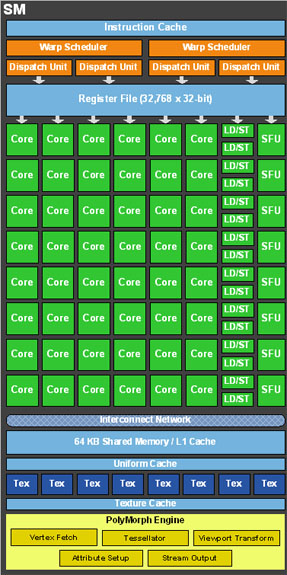
\includegraphics[scale=0.35]{embed-arch2.jpg}  
    \end{column}
    \begin{column}{.5\textwidth}
      A GPU é subdividida em vários Streaming Multiprocessor, como o do lado, que agrupam 48 processadores.
    \end{column}
  \end{columns}
\end{frame}

%-------------------------------------
\section{Comparação entre as linguagens}
%-------------------------------------

\frame{
  \frametitle{Termos Técnicos}
  A explicação dos termos técnicos que serão usados:
  \begin{itemize}
    \item[Kernel] Função que será executada em cada processador da placa de vídeo.
    \item[Host]   Programa que tem a função de preparar o ambiente para o kernel e iniciá-lo na GPU.
    \item[SIMD]   \textit{Single Instrution, Multiple Data}. As GPU executam suas tarefas usando esse paradigma.
    \item[Device]   Hardware onde os kernels serão executados, normalmente uma GPU ou CPU.
  \end{itemize}
}

\frame{
  \frametitle{Semelhanças}
  Alguns elementos são iguais para as duas linguagens.
  \begin{itemize}
    \item Para iniciar a execução num device é necessario que um programa chamado de host inicie o ambiente de execução na GPU.
    \item As threads executando no device são identificadas por indices.
    \item As threads são agrupadas em conjuntos antes de serem enviadas para execução no device.
    \item A alocação e preenchimento da memória no device é controlada pelo host.
  \end{itemize}
}

\frame{
  \frametitle{Semelhanças}
  \begin{itemize}
    \item A execução dos kernels podem ser síncronas ou assíncronas com o a execução do host.
    \item As duas linguagens definem versões tanto para os hardwares como para as APIs que elas usam.
  \end{itemize}
}

\frame{
  \frametitle{Semelhanças}
  \begin{itemize}
      \item Existem 4 locais diferentes para a memória que é enviada para o device:
        \begin{enumerate}
         \item Global Memory  - Toda e qualquer thread tem acesso a essa memória.
         \item Constat Memory - Memória que permanece fixa ao andar da execução.
         \item Local Memory   - Região da memória dividida pelas threads de um mesmo SM.   
         \item Private Memory - Região privada para cada thread.
       \end{enumerate} 
  \end{itemize}
}

\frame{
  \frametitle{Diferenças - Plataforma}
  No OpenCL, a inicialização de um device é de responsabilidade do programador.\\
  No CUDA, esse processo é feito por diretivas.
}

\frame{
  \frametitle{Diferenças - Plataforma}
  No OpenCL existem 2 tipos de execução diferentes:
  \begin{enumerate}
    \item Data Parallel
    \item Task Parallel
  \end{enumerate}
  O CUDA implementa o modelo SIMT (\textit{Single Instruction, Multiple Thread}).
}

\frame{
  \frametitle{Diferenças - Execução}
  \begin{itemize}
    \item Parecido entre elas, já que está ligado ao hardware da GPU.
    \item Threads são separadas em blocos.
    \item Os blocos são escalonados para execução nos \textbf{SM}.
  \end{itemize}
}

%-------------------------------------
\section{Comparação de Performance}
%-------------------------------------

\frame{
  \frametitle{Ideia}
  Para comparar a performance das duas linguagens foram usados dois tipos de kernel, um em que o desempenho está ligado ao acesso a
  memória (memory bound) e outro que está ligado à velocidade de processamento (compute bound).
}

\frame{
  \frametitle{Kernel Memory bound} 
  Para comparar o acesso a memória, foi usado um kernel que faz a cópia de uma matriz de floats para outras.
} 

\begin{frame}[fragile]
  \frametitle{Kernel Memory Bound}
  \begin{lstlisting}
    __kernel void matrixmulti(__global float* a, 
          __global float* b, 
          __global int* rowSize, 
          __global int* columnSize) {
          
      unsigned int row = get_global_id(0);
      unsigned int column = get_global_id(1);
      
      b[row+column*(*rowSize)] 
          = a[row+column*(*rowSize)];
    }
  \end{lstlisting}
\end{frame}

\frame{
  \frametitle{Kernel Compute bound}
  Para comparar o processamento, um kernel que multiplica duas matrizes de doubles e guarda o valor numa terceira fui usado.
}

\begin{frame}[fragile]
  \frametitle{Kernel Compute bound}
  \begin{lstlisting}
    __kernel void matrixmulti(__global int* a, 
                              __global int* b, 
                              __global int* c, 
                              __global int* size) {
        unsigned row = get_global_id(0);
        unsigned column = get_global_id(1);
        unsigned i;
        
        row *= (*size);
        c[row+column] = 0;
        for( i = 0; i < (*size); i++ ) 
            c[row+column] += 
                a[row+i]*b[i*(*size)+column];
    }
  \end{lstlisting}
\end{frame}

\begin{frame}[fragile]
  \frametitle{Estatistica Memory bound}
  \begin{columns}
    \begin{column}{.5\textwidth}
          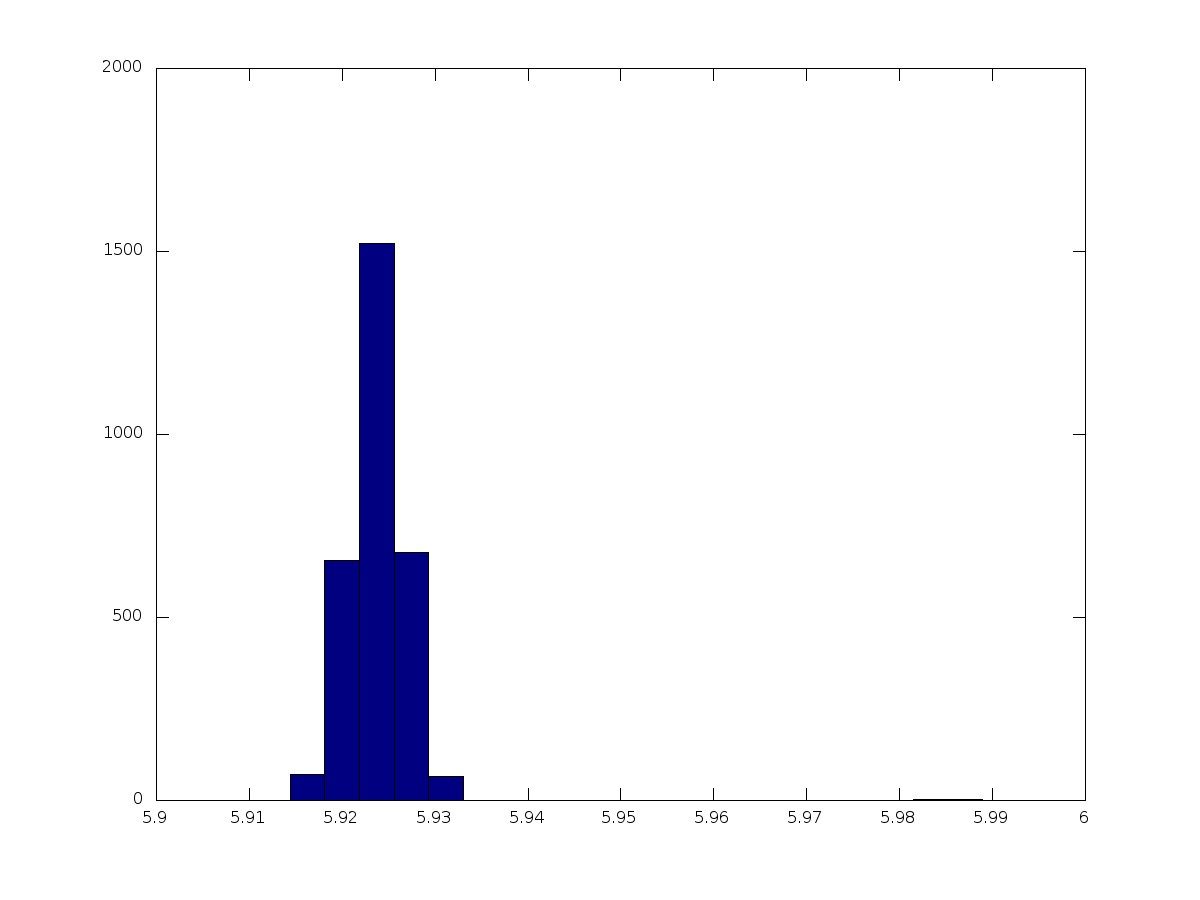
\includegraphics[scale=0.15]{resultados_cuda_memory_histo.jpg} \\
          CUDA
    \end{column}
    \begin{column}{.5\textwidth}
          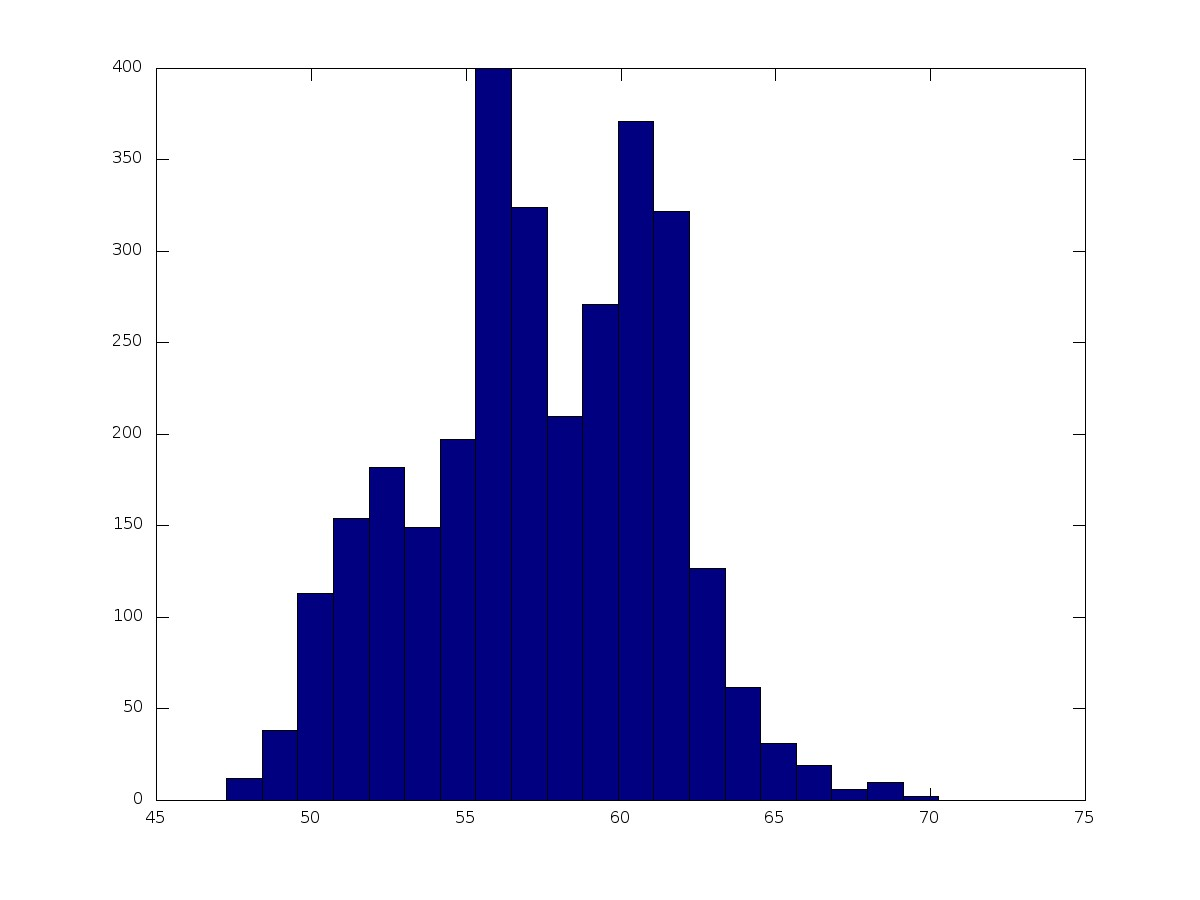
\includegraphics[scale=0.15]{resultados_opencl_memory_histo.jpg} \\
          OpenCL
    \end{column}
  \end{columns}
\end{frame}

\begin{frame}[fragile]
  \frametitle{Estatistica Process bound}
  \begin{columns}
    \begin{column}{.5\textwidth}
      \begin{figure}
          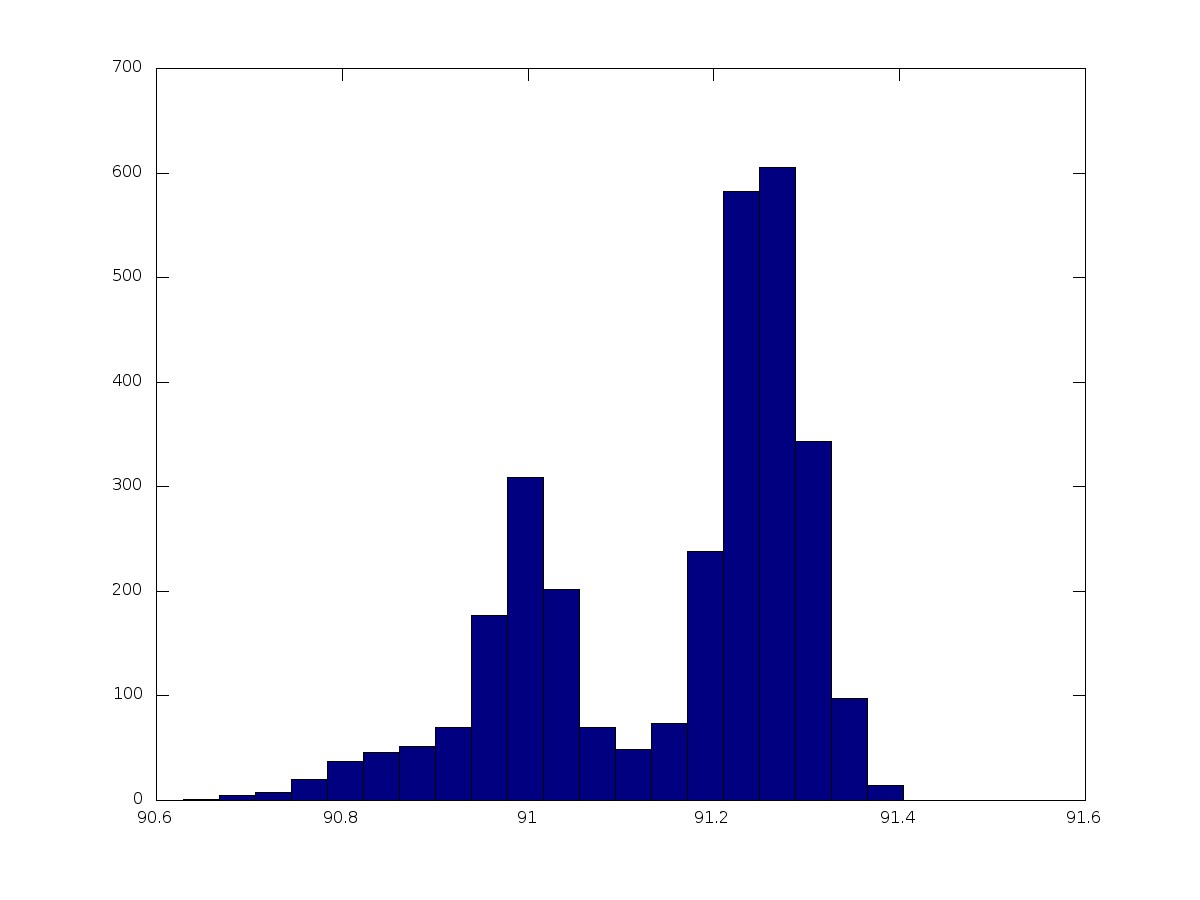
\includegraphics[scale=0.15]{resultados_cuda_process_histo.jpg} \\
          CUDA        
      \end{figure}
    \end{column}
    \begin{column}{.5\textwidth}
      \begin{figure}
          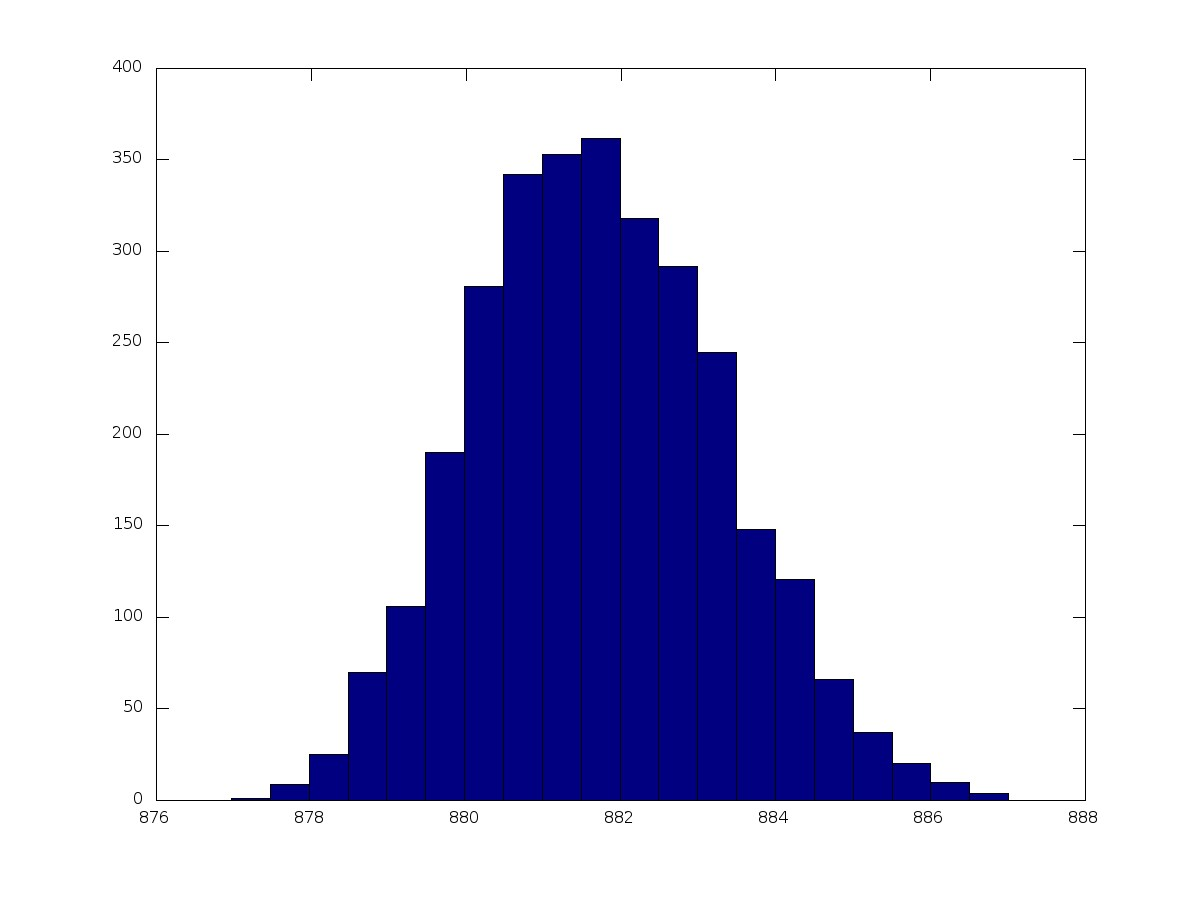
\includegraphics[scale=0.15]{resultados_opencl_process_histo.jpg} \\
          OpenCL
      \end{figure}
    \end{column}
  \end{columns}
\end{frame}

\frame{
  \frametitle{Explicação dos PTX}
  Para melhorar a compatibilidade dos programas rodando em GPUs diferentes, 
  a NVIDIA implementou uma máquina virtual, a Parallel Thread Execution (PTX). 
}

\begin{frame}[fragile]
  \frametitle{Arquivo .ptx}
  Exemplo de um arquivo .ptx:
  \begin{lstlisting}
  mov.u32 	%r2, %ntid.x;
	  mov.u32 	%r3, %ctaid.x;
	  mov.u32 	%r4, %tid.x;
	  mad.lo.s32 	%r10, %r2, %r3, %r4;
	  
	  mov.u32 	%r5, %ntid.y;
	  mov.u32 	%r6, %ctaid.y;
	  mov.u32 	%r7, %tid.y;
	  mad.lo.s32 	%r11, %r5, %r6, %r7;
  \end{lstlisting}
\end{frame}

\begin{frame}[fragile]
  \frametitle{Comparação dos PTX}
  Pelos .ptx é possível verificar algumas das diferenças entre as abstrações das linguagens:
  \begin{enumerate}
    \item O OpenCL usa um registrador a mais que o CUDA para calcular o indice de uma thread.
    \item O OpenCL faz mais leituras da memória padrão que o CUDA. 
  \end{enumerate}
\end{frame}

\begin{frame}
  \frametitle{Comparação dos PTX}
  Pelos resultados dos .ptx, é evidente que o compilador para PTX do CUDA é mais otimizado que o do OpenCL. \\
\end{frame}


\end{document}
